%
% Modelo de trabalho acadêmico
% Documento principal
%
% Centro Federal de Educação Tecnológica de Minas Gerais - CEFET-MG
% Autor: Cristiano Fraga G. Nunes <cfgnunes@gmail.com>
%
%
% Projeto hospedado em: https://github.com/cfgnunes/latex-cefet-mg
%

% Largura da tabulação dos arquivos igual a 8 (utilizar 'Tab' ao invés de 'Espaços')
% TODO: criar glossário
% TODO: criar índice remissivo

\documentclass{abntex2-cefetmg}

% importações de pacotes
	\usepackage[alf, abnt-emphasize=bf, bibjustif, recuo=0cm, abnt-etal-cite=2, abnt-etal-list=0]{abntex2cite}	% citações padrão ABNT
	\usepackage{bookmark}					% cria menu de bookmarks
	\usepackage[utf8]{inputenc}				% acentuação direta
	\usepackage[T1]{fontenc}				% codificação da fonte em 8 bits
	\usepackage[dvips]{graphicx}				% inserir figuras
	\usepackage{subfig}					% posicionamento de figuras
	\usepackage{amsfonts, amssymb, amsmath, dsfont}		% fonte e simbolos matemáticos
	\usepackage{booktabs}					% comandos para tabelas
	\usepackage{verbatim}					% texto é interpretado como escrito no documento
	\usepackage{multirow, array}				% múltiplas linhas e colunas em tabelas
	\usepackage[bottom]{footmisc}				% mantem as notas de rodapé sempre na mesma posicao
	\usepackage{indentfirst}				% indenta o primeiro parágrafo de cada seção.
	\usepackage{microtype}					% para melhorias de justificação?
	\usepackage{times}					% usa a fonte Times
	%\usepackage{lmodern}					% usa a fonte Latin Modern
	%\usepackage[algoruled, portuguese]{algorithm2e}	% escrever algoritmos
	%\usepackage{acronym}					% produzir acrônimos
	%\usepackage{scalefnt}					% permite redimensionar tamanho da fonte
	%\usepackage{color, colortbl}				% comandos de cores
	%\usepackage{lscape}					% permite páginas em modo "paisagem"
	%\usepackage{breakurl}					% permite quebra de linha em urls
	%\usepackage{ae,aecompl}				% fontes de alta qualidade
	%\usepackage{picinpar}					% dispor imagens em parágrafos
	%\usepackage{latexsym}					% simbolos matematicos
	%\usepackage{upgreek}					% fonte letras gregas
	%\usepackage{dsfont}					% fonte matematica
	%\usepackage{type1ec}					% fonte Times
	%\usepackage{pxfonts}					% fonte
	%\usepackage{palatino}					% fonte palatino
	%\usepackage{psfrag}					% símbolos latex em figuras eps
	%\usepackage{subeqnarray}				% sub enumeração de equações
	%\usepackage{bibentry}					% uso de bibtex inline
	%\usepackage{makeidx}					% produzir índice remissivo (glossario)
	%\usepackage{multind}					% produzir índices múltiplos

% inclui o prêambulo do documento
	%
% Documento: Preâmbulo
%

% nome da instituicao
\instituicao{Centro Federal de Educação Tecnológica de Minas Gerais}

% nome do programa
%\programa{Curso de Engenharia de Computação}

% nome do departamento
%\departamento{Departamento de Computação}

% área
%\area{Área de concentração}

% Dissertação, Tese, Monografia
\tipotrabalho{Monografia}

% Mestre, Doutor, Engenheiro
%\titulacao{Engenheiro de Computação}

% titulo do trabalho em portugues
\titulo{Título do Trabalho}

% subtitulo do trabalho em portugues, se houver
%\subtitulo{Subtítulo do Trabalho}

% titulo do trabalho em ingles
%\title{Title in English}

% autor do trabalho
\autor{Nome do acadêmico}
%\autordois{Nome do segundo autor}
%\autortres{Nome do terceiro autor}
%\autorquatro{Nome do quarto autor}
%\autorcinco{Nome do quinto autor}
%\autorseis{Nome do sexto autor}
%\autorsete{Nome do sétimo autor}

% palavras-chave do trabalho
%\palavraschave{Palavra-chave 1, Palavra-chave 2, ...}

% palavras-chave do trabalho em ingles
%\keywords{Keyword 1, Keyword 2, ...}

%\comentario{\DOCdocumentodata{} apresentada ao \DOCprogramadata{} do \ABNTinstituicaodata{}, como requisito parcial para obtenção do grau de \DOCtitulacaodata{}.}

% nome do orientador do trabalho
%\orientador{Nome do orientador}
%\orientador[Orientadora:]{Nome da orientadora}

% nome do co-orientador do trabalho, caso exista
%\coorientador{Nome do co-orientador}
%\coorientador[Co-orientadora:]{Nome da co-orientadora}

% no caso de 2 co-orientadores, usar esta sintaxe
%\coorientador[Co-orientadores:]{Nome do co-orientadorA}
%\coorientadorb{Nome do co-orientadorB}

% local
\local{Belo Horizonte}

% data
\data{2014}

% texto da folha de apresentação
%\textoaprovacao{\DOCdocumentodata{} julgada e aprovada, para a obtenção do grau de \DOCtitulacaodata{} no \DOCprogramadata{}.}

% data da folha de aprovação
%\localdia{Belo Horizonte, 23 de janeiro de 2014}

% nome da primeira pessoa a assinar a folha de apresentação
%\primeiroassina{Prof. Dr. A \\ Instituição}

% nome da segunda pessoa (se houver) a assinar a folha de apresentação
%\segundoassina{Professor B \\ Instituição}

% nome da terceira pessoa (se houver) a assinar a folha de apresentação
%\terceiroassina{Professor C \\ Instituição}

% nome da quarta pessoa (se houver) a assinar a folha de apresentação
%\quartoassina{Professor D \\ Instituição}


% hifenização de palavras desconhecidas
%	\hyphenation{
%		Na-ra-ya-nan
%		qua-dros-cha-ves
%		Bras-nett
%		Kat-sa-gge-los
%	}

% define as cores dos links e informações do pdf
\makeatletter
\hypersetup{
	colorlinks,
	linkcolor=black,
	citecolor=black,
	filecolor=black,
	urlcolor=black,
	breaklinks=true,
	pdftitle={\@title},
	pdfauthor={\@author},
	pdfsubject={\imprimirpreambulo},
	pdfkeywords=pdfkeywords={abnt}{latex}{abntex}{abntex2}{trabalho acadêmico}
}
\makeatother

% início do documento
\begin{document}

% Retira espaço extra obsoleto entre as frases.
\frenchspacing 

% elementos pré textuais
	\pretextual
	\imprimircapa						% Capa
	\imprimirfolhaderosto					% Folha de rosto

	%
% Documento: Folha de aprovação
%

\begin{folhadeaprovacao}

	\begin{center}
		{\large\normalfont\scshape\textbf\imprimirautor}

		\vspace*{\fill}\vspace*{\fill}
		\begin{center}
			\ABNTEXchapterfont\Large\scshape\imprimirtitulo
		\end{center}
		\vspace*{\fill}

		\hspace{.45\textwidth}
		\begin{minipage}{.5\textwidth}
			\imprimirpreambulo
		\end{minipage}
		\vspace*{\fill}
	\end{center}

	\begin{center}
		Trabalho aprovado. \imprimirlocal, 24 de novembro de 2014
	\end{center}

	\assinatura{\textbf{\imprimirorientador} \\ Orientador} 
	\assinatura{\textbf{Professor} \\ Convidado 1}
	\assinatura{\textbf{Professor} \\ Convidado 2}
	%\assinatura{\textbf{Professor} \\ Convidado 3}
	%\assinatura{\textbf{Professor} \\ Convidado 4}

	\begin{center}
		\normalfont\scshape\normalsize{\imprimirlocal}\\
		\normalfont\scshape\normalsize{\imprimirdata}
	\end{center}

\end{folhadeaprovacao}
	% Folha de aprovação
	%
% Documento: Dedicatória
%

\begin{dedicatoria}
Espaço reservado para dedicatória.
Inserir seu texto aqui...
\end{dedicatoria}

		% Dedicatória
	%
% Documento: Agradecimentos
%

\begin{agradecimentos}

Inserir seu texto aqui...

\end{agradecimentos}

	% Agradecimentos
	%
% Documento: Epígrafe
%

\begin{epigrafe}

\textit{``O fator decisivo para vencer o maior obstáculo é, invariavelmente, ultrapassar o obstáculo anterior.'' (Henry Ford)}

\end{epigrafe}
		% Epígrafe
	%
% Documento: Resumo (Português)
%

\begin{resumo}

 O resumo deve ressaltar o
 objetivo, o método, os resultados e as conclusões do documento. A ordem e a extensão
 destes itens dependem do tipo de resumo (informativo ou indicativo) e do
 tratamento que cada item recebe no documento original. O resumo deve ser
 precedido da referência do documento, com exceção do resumo inserido no
 próprio documento. (\ldots) As palavras-chave devem figurar logo abaixo do
 resumo, antecedidas da expressão Palavras-chave:, separadas entre si por
 ponto e finalizadas também por ponto.

\textbf{Palavras-chaves}: latex. abntex. editoração de texto.

\end{resumo}
		% Resumo na língua vernácula
	%
% Documento: Resumo (Inglês)
%

\begin{abstract}
Inserir seu texto aqui... (máximo de 500 palavras)
\end{abstract}
		% Resumo em língua estrangeira
	%
% Documento: Lista de ilustrações
%

\pdfbookmark[0]{\listfigurename}{lof}
\listoffigures*
\cleardoublepage
	% Lista de ilustrações
	%\listadequadros					% Lista de quadros
	%
% Documento: Lista de tabelas
%

\pdfbookmark[0]{\listtablename}{lot}
\listoftables*
\cleardoublepage
		% Lista de tabelas
	%
% Documento: Lista de abreviaturas e siglas
%

\begin{siglas}
  \item[Fig.] Area of the $i^{th}$ component
  \item[456] Isto é um número
  \item[123] Isto é outro número
  \item[lauro cesar] este é o meu nome
\end{siglas}
		% Lista de abreviaturas e siglas
	%
% Documento: Lista de símbolos
%

\begin{simbolos}
  \item[$ \Gamma $] Letra grega Gama
  \item[$ \Lambda $] Lambda
  \item[$ \zeta $] Letra grega minúscula zeta
  \item[$ \in $] Pertence
\end{simbolos}
	% Lista de símbolos
	%
% Documento: Sumário
%

\pdfbookmark[0]{\contentsname}{toc}
\tableofcontents*
\cleardoublepage		% Sumário

% elementos textuais
	\textual
	%
% Documento: Introdução
%

\chapter{Introdução}\label{chap:introducao}

O presente documento é um exemplo de uso do estilo de formatação LATEX elaborado para atender às Normas para Elaboração de Trabalhos Acadêmicos. O estilo de formatação {\ttfamily abnt-cefetmg.cls} tem por base o pacote ABNTEX -- cuja leitura da documentação \cite{abnTeX2009} é fortemente sugerida.

Para melhor entendimento do uso do estilo de formatação, aconselha-se que o potencial usuário analise os comandos existentes no arquivo {\ttfamily main.tex} e os resultados obtidos no arquivo {\ttfamily main.pdf} depois do processamento pelo software LATEX + BIBTEX \cite{LaTeX2009,BibTeX2009}. Recomenda-se a consulta ao material de referência do software para a sua correta utilização \cite{Lamport1986,Buerger1989,Kopka2003,Mittelbach2004}.

\section{Motivação}
\label{sec:motivacao}

Uma das principais vantagens do uso do estilo de formatação para LATEX é a formatação \textit{automática} dos elementos que compõem um documento acadêmico, tais como capa, folha de rosto, dedicatória, agradecimentos, epígrafe, resumo, abstract, listas de figuras, tabelas, siglas e símbolos, sumário, capítulos, referências, etc. Outras grandes vantagens do uso do LATEX para formatação de documentos acadêmicos dizem respeito à facilidade de gerenciamento de referências cruzadas e bibliográficas, além da formatação -- inclusive de equações matemáticas -- correta e esteticamente perfeita.

\section{Caracterização do Problema}
\label{sec:caracProblema}

Inserir seu texto aqui...

\section{Objetivos}
\label{sec:objetivos}

\subsection{Objetivo Geral}
\label{subsec:objetivoGeral}

Prover um modelo de formatação LATEX que atenda às normas da instituição atual e às normas brasileiras.

\subsection{Objetivos Específicos}
\label{subsec:objetivosEspecificos}

\begin{itemize}
	\item Obter documentos acadêmicos automaticamente formatados com correção e perfeição estética.
	\item Desonerar autores da tediosa tarefa de formatar documentos acadêmicos, permitindo sua concentração no conteúdo do mesmo.
	\item Desonerar orientadores e examinadores da tediosa tarefa de conferir a formatação de documentos acadêmicos, permitindo sua concentração no conteúdo do mesmo.
\end{itemize}


\section{Organização do Documento}
\label{sec:organizacaoDocumento}

Inserir seu texto aqui...

\section{Justificativa}
\label{sec:justificativa}

Inserir seu texto aqui...
		% Introdução
	%
% Documento: Trabalhos Relacionados
%

\chapter{Trabalhos Relacionados}

Este capítulo inclui muitas citações bibliográficas. Os principais
itens de bibliografia citados são livros, artigos em conferências,
artigos em {\textit journals} e páginas Web. A bibliografia deve seguir o
padrão ABNT\footnote{Este não é o endereço oficial da
ABNT pois as Normas Técnicas oficiais são pagas e não estão disponíveis na Web.}.

A bibliografia é feita no padrão {\ttfamily bibtex}.  As referências são
colocadas em um arquivo separado. Os elementos de
cada item bibliográfico que devem constar na bibliografia são
apresentados a seguir.

Para livros, o formato da bibliografia no arquivo fonte é o seguinte:

\begin{verbatim}
    @Book{linked,
      author =       {A. L. Barabasi},
      title =        "{Linked: The New Science of Networks}",
      publisher =    {Perseus Publishing},
      year =         {2002},
    }
\end{verbatim}

A citação deste livro se faz da seguinte forma \verb#\cite{linked}# e o resultado fica assim \cite{linked}.
Para os artigos em {\textit journals}, veja por exemplo \cite{acmsurveys},
descrito da seguinte forma no arquivo {\ttfamily .bib}:

\begin{verbatim}
   @article{acmsurveys,
     author = {Deepayan Chakrabarti and Christos Faloutsos},
     title = {Graph mining: Laws, generators, and algorithms},
     journal = {ACM Computing Surveys},
     volume = {38},
     number = {1},
     year = {2006},
     pages = {2-59},
     publisher = {ACM},
     address = {New York, NY, USA},
   }
\end{verbatim}

O artigo \cite{3faloutsos} foi publicado em conferência.  Embora
às vezes seja difícil distinguir um artigo publicado em {\textit
  journal} de um artigo publicado em conferência, esta distinção é
fundamental.  Em caso de dúvida, procure ajuda de seu orientador.

Veja também duas citações juntas \cite{rp99,mar00}  e como citar
endereços Web \cite{irl:06}. 
O trabalho realizado para editar as citações no formato correto é
compensado por uma bibliografia impecável.
	% Trabalhos relacionados
	%
% Documento: Fundamentação Teórica
%

\chapter{Fundamentação Teórica}
\label{chap:fundamentacaoTeorica}

A seguir ilustra-se a forma de incluir figuras, tabelas, equações, siglas e símbolos no documento, obtendo indexação automática em suas respectivas listas. A numeração sequencial de figuras, tabelas e equações ocorre de modo automático. Referências cruzadas são obtidas através dos comandos \verb#\label{}# e \verb#\ref{}#. Por exemplo, não é necessário saber que o número deste capítulo é \ref{chap:fundamentacaoTeorica} para colocar o seu número no texto. Isto facilita muito a inserção, remoção ou relocação de elementos numerados no texto (fato corriqueiro na escrita e correção de um documento acadêmico) sem a necessidade de renumerá-los todos.

Este modelo prove um arquivo \textit{makefile}, portanto, para gerar este documento no formato PDF, basta apenas executar o comando {\ttfamily make all} no linux. Para limpar os arquivos temporários, basta digitar o comando {\ttfamily make clean}.

\section{Figuras e gráficos}
\label{sec:figuras}

Abaixo é apresentado um exemplo de figura e de gráfico. A figura \ref{fig:kdtree} aparece automaticamente na lista de figuras e o gráfico \ref{chr:buscaimg} aparece automaticamente na lista de gráficos. Para uso avançado de imagens no LATEX, recomenda-se a consulta de literatura especializada \cite{Goossens2007}.

\begin{figure}[!htb]
	\centering
	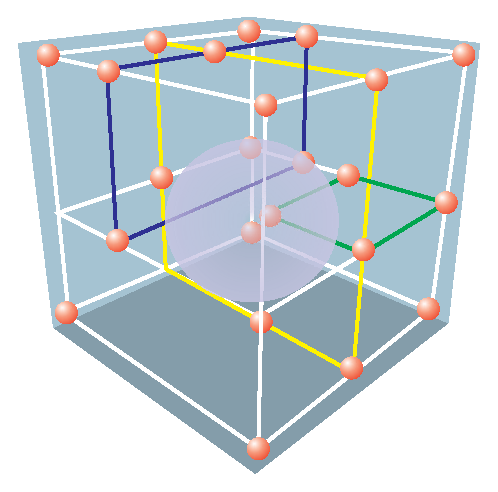
\includegraphics[width=0.3\textwidth]{./figuras/figkdtree.eps}
	\caption{Exemplo da estrutura de uma árvore KD}
	\fonte{\cite{CELSO2012}}
	\label{fig:kdtree}
\end{figure}

\begin{grafico}[!htb]
	\centering
	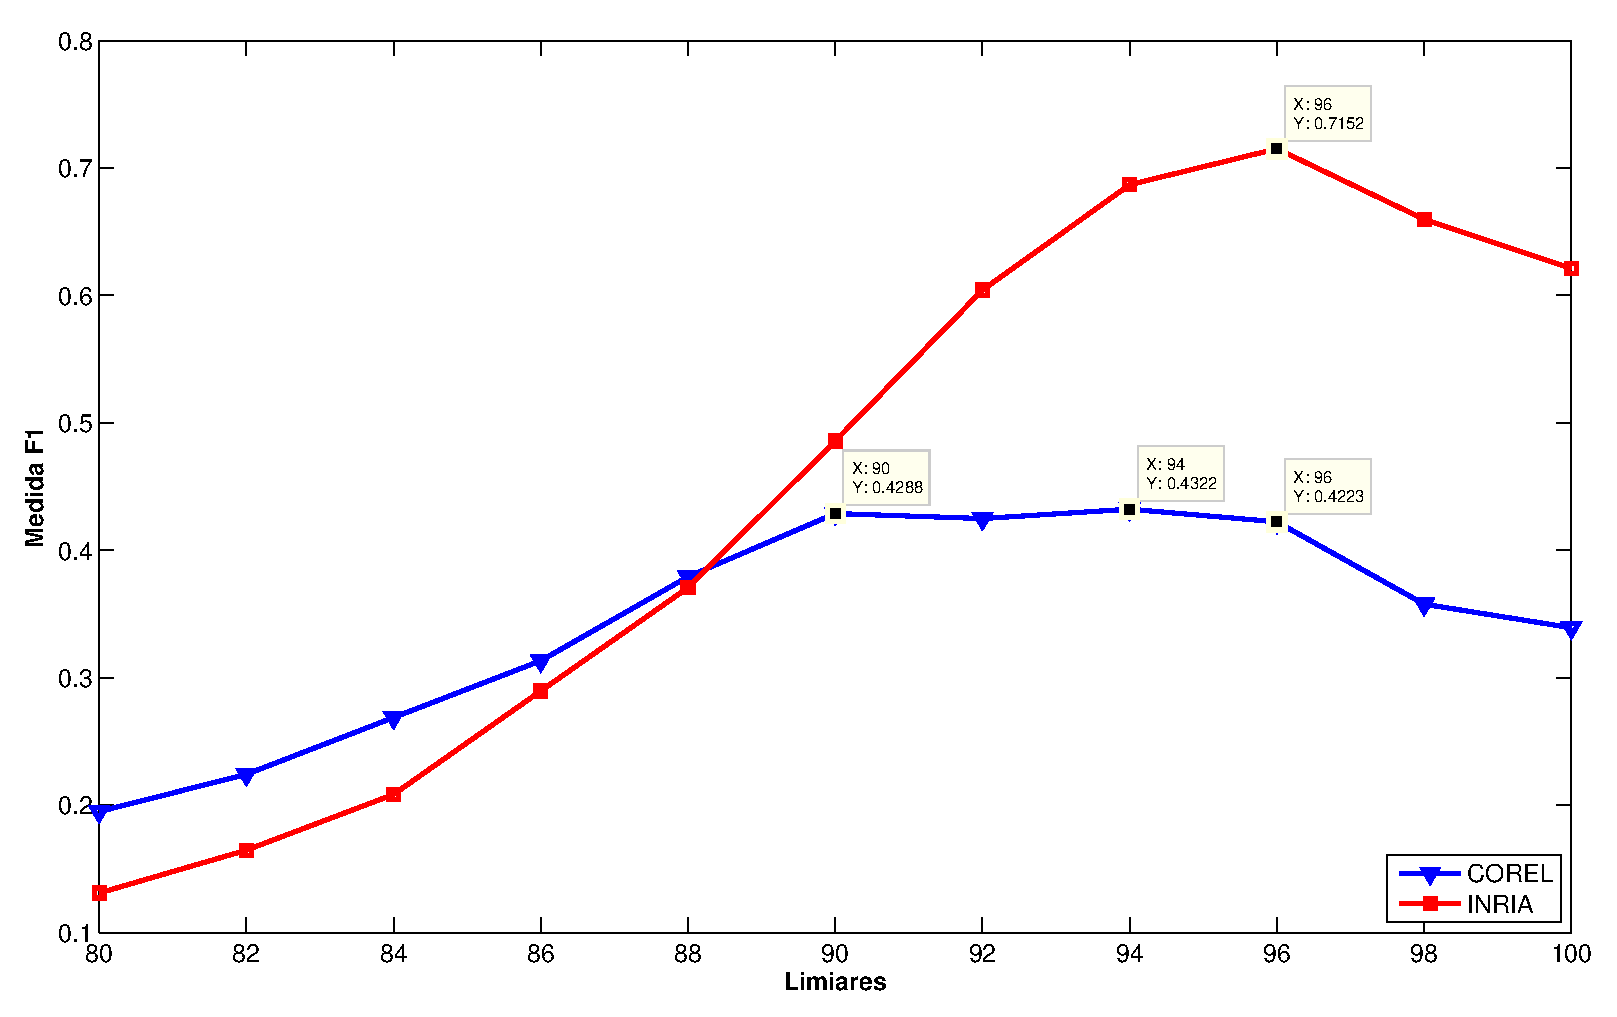
\includegraphics[width=0.7\textwidth]{./graficos/buscaimg.eps}
	\caption[Resultado da busca por imagem]{Resultado da busca por imagem.}
	\label{chr:buscaimg}
\end{grafico}

\section{Quadros e Tabelas}
\label{sec:tabelas}

Também é apresentado o exemplo do quadro \ref{qua:vertices} e da tabela \ref{tab:correlacao}, que aparece automaticamente na lista de tabelas. Informações sobre a construção de tabelas no LATEX podem ser encontradas na literatura especializada \cite{Lamport1986,Buerger1989,Kopka2003,Mittelbach2004}.

\begin{quadro}[!htb]
	\centering
	\begin{tabular}{|c|c|c|} \hline
		\multirow{2}{32mm}{Vértices Retirados} &\multicolumn{2}{|c|}{Componentes Excluídos} \\ \cline{2-3}
		&Quantidade &Vértices do maior componente\\ \hline\hline
		Original &0        &- \\ \hline
		1\%      &4        &3 \\ \hline
		5\%      &14       &3 \\ \hline
		10\%     &31       &5 \\ \hline
		20\%     &66       &5 \\ \hline
		30\%     &94       &5 \\ \hline
		40\%     &110      &5 \\ \hline
		50\%     &166      &5 \\ \hline
		75\%     &352      &6 \\ \hline
		90\%     &688      &19 \\ \hline
	\end{tabular}
	\caption[Componentes desconectados na remoção híbrida]{Componentes desconectados na remoção híbrida\label{qua:vertices}}
\end{quadro}


Muitos confundem, mas existe diferença entre tabelas e quadros.
Um quadro é formado por linhas horizontais e verticais,
sendo, portanto ``fechado''. Normalmente é usado
para apresentar dados secundários. Nada impede, porém,
que um quadro apresente resultados da pesquisa.
Um quadro normalmente apresenta resultados
qualitativos (textos). O número do quadro e o título
vêm acima do quadro, e a fonte, deve vir abaixo.
Uma tabela é formada apenas por linhas verticais, sendo,
portanto ``aberta''. Normalmente é usada para
apresentar dados primários, e geralmente vem nos
“resultados” e na discussão do trabalho. Nada
impede, porém, que uma tabela seja usada no
referencial teórico de um trabalho. Uma tabela
normalmente apresenta resultados quantitativos
(números). O número da tabela e o título vêm
acima da tabela, e a fonte, deve vir abaixo, como
no quadro.

Exemplos de tabelas:

\begin{table}[!htb]
	\centering
	\caption[Correlação de valores x e y]{Exemplo de uma tabela mostrando a correlação entre x e y.\label{tab:correlacao}}
	\begin{tabular}{cc}
		\hline 
		x & y \\
		\hline
		1 & 2 \\
		3 & 4 \\
		5 & 6 \\
		7 & 8 \\
		\hline 
	\end{tabular}
	\fonte{Autoria própria.}
\end{table}


\begin{table}[!htb]
	\centering
	\begin{tabular}{rrrrr}
		\toprule
			& Valores 1 & Valores 2 & Valores 3 & Valores 4 \\
		\midrule
			Caso 1 & 0,86 & 0,77 & 0,81 & 163 \\
			Caso 2 & 0,19 & 0,74 & 0,25 & 180 \\
			Caso 3 & 1,00 & 1,00 & 1,00 & 170 \\
		\bottomrule
	\end{tabular}
	\caption[Resultado dos testes]{Resultado dos testes.\label{tab:testes}}
\end{table}


\section{Equações}
\label{sec:equacoes}

A transformada de Laplace é dada na equação (\ref{eq:laplace}), enquanto a equação (\ref{eq:dft}) apresenta a formulação da transformada discreta de Fourier bidimensional\footnote{Deve-se reparar na formatação esteticamente perfeita destas equações.}.

\begin{equation}
	X(s) = \int\limits_{t = -\infty}^{\infty} x(t) \, \text{e}^{-st} \, dt
	\label{eq:laplace}
\end{equation}

\begin{equation}
	F(u, v) = \sum_{m = 0}^{M - 1} \sum_{n = 0}^{N - 1} f(m, n) \exp \left[ -j 2 \pi \left( \frac{u m}{M} + \frac{v n}{N} \right) \right]
	\label{eq:dft}
\end{equation}

\section{Siglas e símbolos}
\label{sec:siglas}

O pacote ABNTEX permite ainda a definição de siglas e símbolos com indexação automática através dos comandos \verb#\sigla{}{}# e \verb#\simbolo{}{}#. Por exemplo, o significado das siglas \sigla{ABNT}{Associação Brasileira de Normas Técnicas} e \sigla{DECOM}{Departamento de Computação} aparecem automaticamente na lista de siglas, bem como o significado dos símbolos\simbolo{$\lambda$}{comprimento de onda},\simbolo{$v$}{velocidade} e\simbolo{$f$}{frequência}aparecem automaticamente na lista de símbolos. Mais detalhes sobre o uso destes e outros comandos do ABNTEX são encontrados em sua documentação específica\cite{abnTeX2009}.

%\section{Algoritmos}
%\label{sec:algoritmos}
%
%Os algoritmos devem ser feitos segundo o modelo abaixo.
%Para isso, utilizar o pacote  {\ttfamily algorithm2e} no início do arquivo principal como neste exemplo.
%
%\begin{algorithm}
%\KwIn{o número $n$ de vértices a remover, grafo original $G(V, E)$}
%\KwOut{grafo reduzido $G'(V,E)$}
% $removidos \leftarrow 0$ \\
% \While {removidos $<$ n } {
%   $v \leftarrow$ Random$(1, ..., k) \in V$ \\
%     \For {$u \in adjacentes(v)$} {
%	remove aresta (u, v)\\
%	$removidos \leftarrow removidos + 1$\\
%     }
%     \If {há  componentes desconectados} {
%	remove os componentes desconectados\\
%     }
%   }
%\caption{Algoritmo para remoção aleatória de vértices}
%\end{algorithm}
	% Fundamentação teórica
	%
% Documento: Metodologia
%

\chapter{Metodologia}

Inserir seu texto aqui...

\section{Delineamento da pesquisa}

Inserir seu texto aqui...

\section{Coleta de dados}

Inserir seu texto aqui...

		% Metodologia
	%
% Documento: Resultados
%

\chapter{Análise de Resultados}

Inserir seu texto aqui...

\section{Situação atual}

Inserir seu texto aqui...

\section{Análise dos dados coletados}

Inserir seu texto aqui...

		% Resultados
	%
% Documento: Conclusões
%

\chapter{Conclusões}
\label{chap:conclusoes}

Espera-se que o uso do estilo de formatação LATEX adequado às Normas para Elaboração de Trabalhos Acadêmicos do CEFET-MG ({\ttfamily abnt-cefetmg.cls}) facilite a escrita de documentos no âmbito desta instituição e aumente a produtividade de seus autores. Para usuários iniciantes em LATEX, além da bibliografia especializada já citada, existe ainda uma série de recursos \cite{CTAN2009} e fontes de informação \cite{TeX-Br2009,Wikibooks2009} disponíveis na Internet.

Recomenda-se o editor de textos Kile como ferramenta de composição de documentos em LATEX para usuários Linux. Para usuários Windows recomenda-se o editor TEXnicCenter \cite{TeXnicCenter2009}. O LATEX normalmente já faz parte da maioria das distribuições Linux, mas no sistema operacional Windows é necessário instalar o software MiKTeX \cite{MiKTeX2009}.

Além disso, recomenda-se o uso de um gerenciador de referências como o JabRef \cite{JabRef2009} ou Mendeley \cite{Mendeley2009} para a catalogação bibliográfica em um arquivo BIBTEX, de forma a facilitar citações através do comando \verb#\cite{}# e outros comandos correlatos do pacote ABNTEX. A lista de referências deste documento foi gerada automaticamente pelo software LATEX + BIBTEX a partir do arquivo {\ttfamily refbase.bib}, que por sua vez foi composto com o gerenciador de referências JabRef.

O estilo de formatação LATEX do CEFET-MG e este exemplo de utilização foi elaborado por
\href{mailto:cfgnunes@gmail.com}{Cristiano Fraga Guimarães Nunes},
baseado nos modelos criados por
\href{mdiogo.kuiaski@gmail.com}{Diogo Rosa Kuiaski} e \href{hvieir@utfpr.edu.br}{Hugo Vieira Neto}. Sugestões de melhoria são bem vindas.

\section{Trabalhos Futuros}
\label{sec:trabalhosFuturos}

Inserir seu texto aqui...
		% Conclusões

% elementos pós textuais
	\postextual
	%
% Documento: Referências Bibliográficas
%

\bibliography{./refbase}	% geracao automatica das referencias a partir do arquivo refbase.bib
		% Referências
	%\include{./elementos-pos-textuais/glossario}		% Glossário
	%
% Documento: Apêndice
%

\apendice
\chapter{Nome do apêndice}
\label{chap:apendicex}

Inserir seu texto aqui...

\chapter{Nome do apêndice}
\label{chap:apendicey}

Inserir seu texto aqui...
		% Apêndices
	%
% Documento: Anexos
%

\anexo
\chapter{Nome do anexo}
\label{chap:anexox}

Inserir seu texto aqui...

\chapter{Nome do anexo}
\label{chap:anexoy}

Inserir seu texto aqui...
		% Anexos
	%\include{./elementos-pos-textuais/indices}		% Índices

\end{document}
